\documentclass[12pt]{article}
\usepackage[a4paper,margin=1in,footskip=0.25in]{geometry} % set margins
\usepackage[portuguese]{babel}
\usepackage[utf8]{inputenc}
\usepackage{hyperref} 
\usepackage{amsmath}
\usepackage{amssymb}
\usepackage{amsthm}
\usepackage{graphicx}    % needed for include graphics
\usepackage{indentfirst}
\usepackage{float}       % needed for [H] figure placement option
\usepackage{setspace}    % needed for doublespacing
\usepackage{tikz}

% Macros
\renewcommand{\familydefault}{\sfdefault} % sans-serif
\newcommand{\lowtext}[1]{$_{\text{#1}}$}

% Adds ./figures/ to the path of figures
\graphicspath{./figures/}

\title{Arquitetura do Console Nintendo 64}
\author{Antônio Augusto Abello, Gustavo Estrela de Matos, Lucas Romão
Silva}

\begin{document}
% Espaçamento duplo 
\doublespacing
\begin{titlepage}
    \vfill
    \begin{center}
        \vspace{0.5\textheight}
        \noindent
        Instituto de Matemática e Estatística \\
        Monografia dos curso Organização de Computadores \\
        \vfill
        \noindent
        {\Large Arquitetura do Console Nintendo 64} \\
        \begin{tabular}{rl}
            {\bf Professor:} & {Siang Wun Song} \\
            {\bf Alunos:}    & {Antônio Augusto Abello} \\
                             & {Gustavo Estrela de Matos} \\
                             & {Lucas Romão Silva} \\
        \end{tabular} \\
        \vspace{\fill}
       \bigskip
        São Paulo, \today \\
       \bigskip
    \end{center}
\end{titlepage}

\pagebreak
\tableofcontents
\pagebreak

\section{Introdução}
\section{Principais Componentes do Nintendo64}
\section{Chip NEC VR4300}
    O chip NEC VR4300 é o principal processador no Nintendo64,
responsável principalmente por processar a lógica dos jogos e, 
também audio. Esse processador foi desenvolvido pela empresa japonesa
NEC e implementa a arquitetura de conjunto de instruções MIPS, 
desenvolvida pela empresa de mesmo nome. A arquitetura MIPS define um
conjunto de instruções do tipo RISC, \emph{reduced instruction set
computer}.

    O processador VR4300 possuia uma arquitetura compatível com 
instruções de 64 bits, apesar de grande parte das instruções do
Nintendo 64 serem de apenas 32 bits. Especificamente nesse console, o
processador da NEC trabalhava a uma frenquência de 93,75 MHz.

\subsection{Principais Componentes do Processador VR4300}
    A figura \ref{fig:vr4300dia} mostra um diagrama com os principais
componentes do processador VR4300 e como eles se comunicam. Nesta seção,
discutiremos o papel de cada um desses componentes.
\begin{itemize}
    \item {\bf System interface} define a interface do chip com os
componentes externos. Essa interface é formada por um bus de 32 bits
e vários outros bits para controle de bits, interrupções, relógio, etc.
No Nintendo  64, algum desses bits se conectam a memória RAM do console
e, também diretamente ao cartucho com o jogo.
    \item {\bf Clock generator} é responsável por determinar o clock
interno do chip, que é o clock do pipeline do processador. Esse 
componente recebe um clock externo e define o clock de pipeline como uma
fração do anterior. Um dos modos de operação do VR4300 é ter o relógio 
interno funcionando com 2 ciclos a cada ciclo do relógio externo.
    \item {\bf Instruction cache} é um cache que guarda a instrução que
está sendo executada. No contexto do pipeline, manter uma cópia da 
instrução lida dentro do processador é essencial para aumentar 
eficiência e permitir operações como desvios e interrupções.
    \item {\bf Execution unit} é uma parte do hardware que é 
especializada em realizar operações aritméticas. Na arquitetura MIPS,
a {\em Execution unit} tem o papel de {\em COP1} (coprocessador 1).
    \item {\bf CP0} é o componente responsável por fazer o controle da
memória (MMU), isto é, permite enderaçemento virtual, controla o acesso
a pedaços de memória diferentes, aloca páginas de memória e outras 
funções. Para ajudar na eficiência de acesso a memória, o {\em} CP0 
possui uma {\em TLB} ({\em Translation Lookaside Buffer}) que é, 
basicamente, um cache para a tradução de endereços virtuais para 
físicos.
    \item {\bf Data cache} é um cache para dados da memória. Os dados 
armazenados nesse componente são indexados pelos endereços virtuais.
Podemos ver, no diagrama, uma conexão entre {\em Execution Unit} e esse 
componente, essa ligação é utilizada quando um dado necessário em uma
computação já está no cache. Quando isso acontece poupamos o trabalho
de buscar dados na memória ou qualquer outro componente pois ele já
está disponível dentro do chip.
    \item {\bf Instruction address} tem o papel de calcular o endereço
da próxima instrução. Esse circuito deve ser capaz de incrementar o
{\em Program Counter}, dando sequência as execuções de instruções, e
também deve ser capaz de atualizar o {\em Program Counter} quando
ocorrem desvios ({\em branch} e {\em jump}).
    \item {\bf Pipeline control} é o circuito que controla a execução
do pipeline do processador. O conceito de pipeline consiste em dividir
a execução de uma tarefa de maneira que mais de uma tarefa possa ser
executada simultaneamente, desde que em diferentes etapas e não 
dependentes. O pipeline do processador VR4300 consiste em cinco etapas
diferentes:
    \begin{itemize}
        \item{IC (Instruction Cache Fetch):} faz a leitura da instrução.
        \item{RF (Register Fetch):} deixa valores de registradores 
prontos para serem usados em cálculos.
        \item{EX (Execution):} executa operações aritméticas.
        \item{DC (Data Cache Fetch):} armazena no cache os dados 
utilizados na instrução.
        \item{WB (Write Back):} atualiza valores na memória ou 
registradores.
    \end{itemize}
O que ocorre em cada etapa do pipeline também depende muito da instrução
que está sendo executada, portanto o que está descrito logo acima é uma
visão superficial de cada uma dessas etapas.
\end{itemize}

\begin{figure}[H]
    \label{fig:vr4300dia}
    \centering
        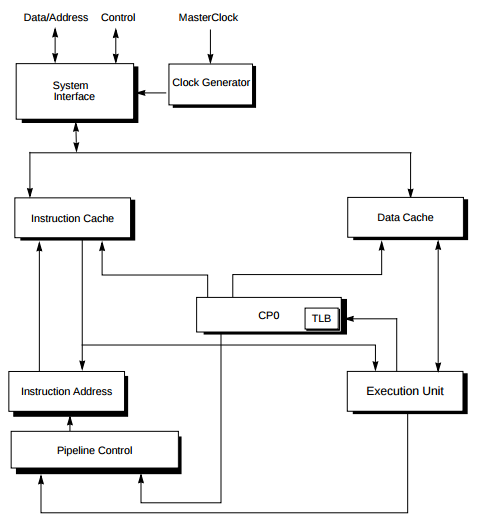
\includegraphics[scale=.65]{figures/vr4300diagram}
    \caption{Um diagrama com os principais componentes do processador 
        VR4300}
\end{figure}

\subsection{Formato de instrução}
    Cada instrução do processador é formada por 32 bits, e elas podem
ser separadas em três categorias: \emph{I-type}, \emph{J-Type} e 
\emph{R-Type}. 

    As intruções do tipo \emph{I-Type} são formadas por 5 bits, $op$,
que determinam a operação; 5 bits em $rs$ e mais 5 em $rt$, que
determinam os registradores que estão sendo operados; e mais 16 bits,
{\em immediate}, que pode representar ou um enderço ou uma constante.
Exemplos de instruções desse tipo são as instruções {\em load} e 
{\em store}.

\begin{figure}[H]
\centering
\begin{tikzpicture}[>=latex, font=\sffamily, every node/.style = 
     {minimum height = 1.5em, outer sep = 0pt, 
     draw=black, fill = blue!20,semithick}]
        \node [minimum width=2cm] 
            at (0,0)    (A) {op};
        \node [anchor=west, minimum width=2cm] 
            at (A.east) (B) {rs};
        \node [anchor=west, minimum width=2cm] 
            at (B.east) (C) {rt};
        \node [anchor=west, minimum width=6cm] 
            at (C.east) (D) {immediate};
        \node [draw=none, fill=none, anchor=west, 
                xshift=2.5cm, yshift=0.75em] 
            at (D.north) (D) {0};
        \node [draw=none, fill=none, anchor=west, 
                xshift=0.25cm, yshift=0.75em] 
            at (C.north) (D) {16};
        \node [draw=none, fill=none, anchor=west, 
                xshift=0.25cm, yshift=0.75em] 
            at (B.north) (D) {21};
        \node [draw=none, fill=none, anchor=west,
                xshift=0.25cm, yshift=0.75em] 
            at (A.north) (D) {26};
        \node [draw=none, fill=none, anchor=west,
                xshift= -1.25cm, yshift=0.75em] 
            at (A.north) (D) {31};
\end{tikzpicture}
\caption{Formato de uma instrução \em{I-Type}} 
\label{fig:instr-itype}
\end{figure}

    As intruções do tipo {\em J-Type} são usadas para controlar o fluxo
do programa. Para isso, esse tipo de instrução pode pular para um 
pedaço específico do código por via de um {\em jump} ou um {\em branch}.
Quando uma instrução do tipo {\em jump} é executada, o desvio sempre 
acontece, ao contrário da instrução {\em branch} na qual é possível 
determinar uma condição para o desvio. No VR4300 essas intruções são
formadas por 5 bits, $op$, que determinam a operação; e mais 26 bits
$target$, que determinam o endereço do possível desvio. Quando a 
instrução é um desvio obrigatório, os 26 bits estão todos disponíveis
para determinar o endereço de destino, mas no caso de um {\em branch}
o valor de $target$ só pode determinar um {\em offset} de 16 bits 
relativo ao registrador {\em PC}.

\begin{figure}[H]
\centering
\begin{tikzpicture}[>=latex, font=\sffamily, every node/.style = 
     {minimum height = 1.5em, outer sep = 0pt, 
     draw=black, fill = blue!20,semithick}]
        \node [minimum width=2cm] 
            at (0,0)    (A) {op};
        \node [anchor=west, minimum width=10cm] 
            at (A.east) (B) {target};
        \node [draw=none, fill=none, anchor=west, 
                xshift=4.75cm, yshift=0.75em] 
            at (B.north) (B) {0};
        \node [draw=none, fill=none, anchor=west, 
                xshift=0.25cm, yshift=0.75em] 
            at (A.north) (A) {26};
\end{tikzpicture}
\caption{Formato de uma instrução \em{J-Type}} \label{fig:instr-jtype}
\end{figure}

    As instruções do tipo {\em R-Type} envolvem apenas o uso de 
registradores. Exemplos de instruções desse tipo são aquelas que
fazem operações aritméticas entre dois registradores e guardam o 
resultado em um terceiro registrador. Essas instruções são formadas
por 5 bits $op$; 5 bits para cada um dos três registradores $rs$, $rt$
e $rd$; 5 bits $sa$ que definem um {\em shift} para o resultado; e mais
6 bits para $function$.

\begin{table}[H]
\centering
\label{r-type-table}
\begin{tabular}{|c|c|}
\hline
Code & Operation \\ \hline
0  & Add \\
1  & Subtract \\
2  & Multiply \\
3  & Divide \\
4  & Square root \\
5  & Absolute value \\
6  & Transfer \\
7  & Sign reverse \\
8  & Convert to 64-bit fixed-point, rounded to nearest/even \\
9  & Convert to 64-bit fixed-point, rounded toward zero \\
10 & Convert to 64-bit fixed-point, rounded to + $\infty$ \\
11 & Convert to 64-bit fixed-point, rounded to – $\infty$ \\
12 & Convert to 32-bit fixed-point, rounded to nearest/even \\
13 & Convert to 32-bit fixed-point, rounded toward zero \\
14 & Convert to 32-bit fixed-point, rounded to + $\infty$ \\
15 & Convert to 32-bit fixed-point, rounded to – $\infty$ \\
16–31 & Reserved \\
32 & Convert to single floating-point \\
33 & Convert to double floating-point \\
34 & Reserved \\
35 & Reserved \\
36 & Convert to 32-bit fixed-point \\
37 & Convert to 64-bit fixed-point \\
38–47 & Reserved \\
8–63 & Floating-point compare \\
\hline
\end{tabular}
\caption{Lista de todas as possíveis funções em uma instrução do tipo
{\em R-Type} \cite{vr4300-datasheet}.}

\end{table}


\section{Chip SGI RCP}


\pagebreak
\begin{thebibliography}{1}
\bibitem{vr4300-datasheet} 
NEC V\lowtext{R}4300, V\lowtext{R}4305, V\lowtext{R}4310 64-bit 
processor User's Manual 7$^{\text{th}}$ edition. Japan, 2000.
\end{thebibliography}

\end{document}


